%!TEX TS-program = xelatex
%!TEX root = ../../maxwell2018thesis.tex

\chapter[General Methodology]{General Methodology}\label{chap:method}

\section{General Methodology Overview}\label{sec:csm:methodology}
In Chapters~\ref{chap:snippets} and~\ref{chap:diversity}, we will be exploring how an individual's searching behaviours (particularly their stopping behaviours) vary under differing contexts. This section provides a high level overview of the \emph{general methodology} that we will employ in these two chapters, focusing on four main tasks:

\begin{itemize}
    \item{conducting a \blueboxbold{user study} to examine real-world searcher behaviours;}
    \item{extracting the \blueboxbold{interaction data and performance measures} from the user study;}
    \item{using the aforementioned data to ground a series of \blueboxbold{simulations} that attempt to replicate the user studies; and}
    \item{\blueboxbold{evaluating} the performance of the simulated users, and \blueboxbold{comparing} the simulated user behaviours against those of their real-world counterparts.}
\end{itemize}

We now discuss each of these different tasks in greater depth, highlighting the key decisions and \todo{assumptions} that we have made. Note that this section is directly applicable to contributory Chapters~\ref{chap:snippets} and~\ref{chap:diversity}; Chapter~\ref{chap:serp} provides an in-depth examination on the realism of the~\gls{acr:csm} before we employ it in the following two contributory chapters. Indeed, given that this chapter relies solely on simulations, we follow the approach followed in Section~\ref{chap:csm:method:simulation} and~\ref{chap:csm:method:evaluation}. However, we do ground our experimentation in Chapter~\gls{acr:csm} with user study interaction data from a following chapter.

% Now that we have outlined the~\gls{acr:csm} and the various stopping strategies that we will operationalise, this section provides a high level explanation of the \emph{general methodology} that we will employ in subsequent contributory chapters of this thesis.
%
%
%
% Now that we have outlined the~\gls{acr:csm} and the various stopping strategies that we will operationalise, this section provides a high level explanation of the general methodology of the subsequent contributory chapters. Chapters~\ref{chap:snippets} and~\ref{chap:diversity} will follow this approach, along with the work detailed in Chapter~\ref{chap:serp}.
%
% In essence, the main aim of the following contributory chapters is to examine what happens to a searcher's behaviours (in particular, their stopping behaviours)
%
%
% ground the data
% ground the simulation
% evaluate it later on
% explore influence of these decision points and stopping strategies under different contexts
%
% We want to examine what happens to a searcher's behaviour when different stopping rules are employed under certain contexts.
% How can we do this? Here, we provide a broad overview of the methodology that was employed in the later chapters of this thesis. Broadly split across two main sections.

\subsection{Test Collection, Topics and Search Engine}\label{sec:csm:methodology:collection}
Central to any~\gls{acr:ir} experiment is a corpus of documents (refer to Section~\ref{sec:ir_background:basics:indexing}) with which subjects participating in the experiment can issue queries against. In conjunction with the document corpus, a number of topics are also used to provide simulated information needs.

For the contributory chapters of this thesis, all work detailed uses the TREC AQUAINT corpus, consisting of over one million news articles from the period ranging 1996 to 2000. All of the news articles were collected from three newswires, namely: the \emph{Associated Press (AP);} the \emph{New York Times (NYT);} and \emph{Xinhua}. More contemporary collections could have been used; the reasons for selecting an older were twofold: \emph{(i)} using such a collection enabled us to easily evaluate the performance of subjects; and \emph{(ii)} employing the AQUAINT corpus provides continuity with a prior line of research using this collection, as shown by~\cite{azzopardi2013query_cost}, for example.

Five topics were also selected from the 50 provided in the \emph{TREC 2005 Robust Track,} as outlined by~\cite{voorhees2006trec_robust}. These topics were selected based upon evidence from a previous user study (of similar nature) conducted by~\cite{kelly2015serp_size}. Evidence showed that the topics offered similar levels of difficulty. The five topics, along with a short description of what constitutes a relevant document, are listed below. These summaries are derived from the TREC topic descriptions that are provided as part of the TREC 2005 Robust Track -- Figure~\ref{fig:topics} illustrates three examples of topic descriptions.

\begin{figure}[t!]
    \centering
    \resizebox{1\hsize}{!}{
    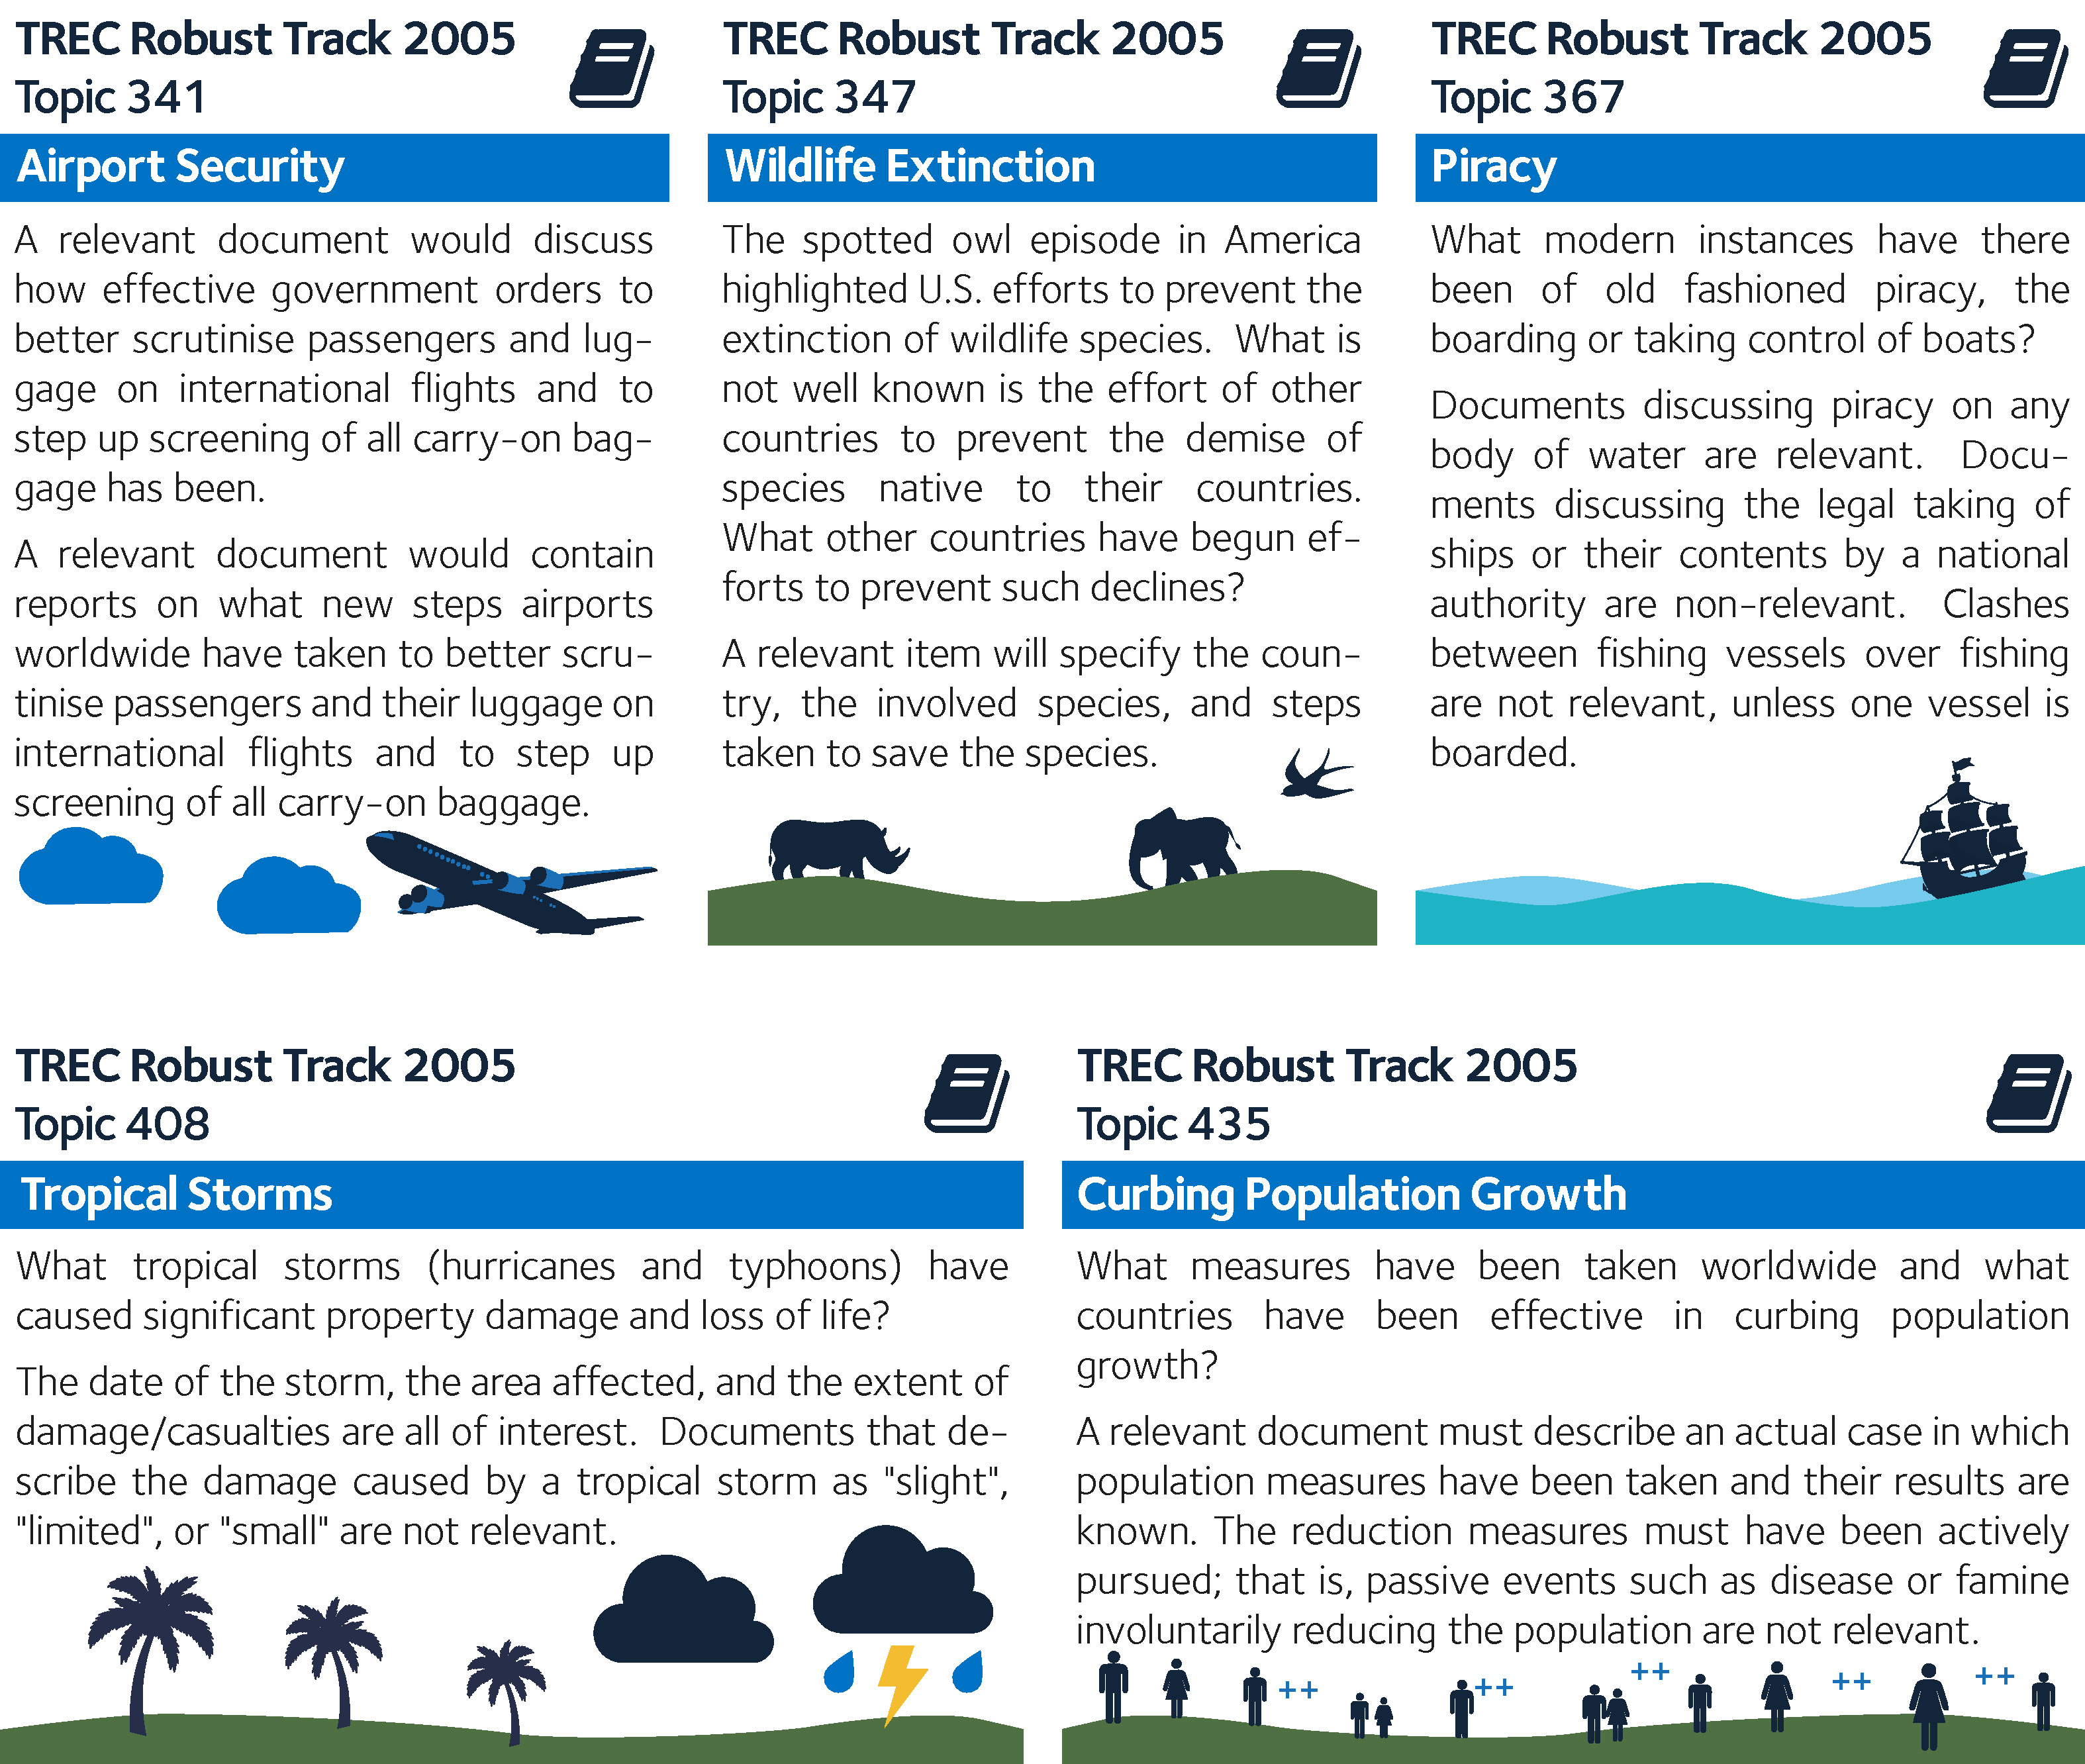
\includegraphics{figures/ch4-topics.pdf}}
    \caption[Examples of TREC Topics]{Three examples of \emph{TREC topic descriptions}, as outlined in Section~\ref{sec:csm:csm:flow}. Topics are extracted from the \emph{TREC 2005 Robust Track,} as outlined by~\cite{voorhees2006trec_robust}. Descriptions provide an explanation as to what constitutes a relevant (and often non-relevant) document.}
    \label{fig:topics}
\end{figure}

\begin{itemize}
    
    \item[]{\blueboxbold{Topic 341 – Airport Security} This topic considers relevant documents as those that discuss additional security measures that were taken by international airports around the world. Relevance is only denoted when a document discusses measures that go beyond the basic passenger and carry-on luggage screening. For example, AQUAINT document \texttt{NYT19980616.0123} discusses \emph{San Francisco International Airport's} attempts at introducing a \emph{robot sniffer,} attempting to look for nitroglycerine in luggage.}
    
    \item[]{\blueboxbold{Topic 347 – Wildlife Extinction} As the title of the topic suggests, this topic concerns wildlife extinction, and what efforts have been taken by countries other than the United States to counter the decline in endangered wildlife. Relevant documents explicitly mention the country, the species of animal, and the efforts the state or other governmental agency took to prevent decline in numbers. For example, document \texttt{XIE20000531.0205} discusses the breeding programme undertaken by China to bolster the number of Siberian Tigers in its jurisdiction.}
    
    \item[]{\blueboxbold{Topic 367 – Piracy} Instances of modern piracy are considered relevant to this topic -- not in the sense of software piracy, but the act of a water going vessel being boarded by individuals wishing to hijack it. Document \texttt{APW19980601.1065} provides an example of this -- the \emph{Petro Ranger}, a large fuel tanker, was boarded by pirates in 1998 in the South China Sea. To be relevant to the topic, the name of the vessel and the body of water it was hijacked on must be mentioned -- those discussing instances of when states intercepted vessels are not relevant.}
    
    \item[]{\blueboxbold{Topic 408 – Tropical Storms} Documents discussing major tropical storms are to be considered relevant, where the storm is reported to have caused significant damage and a large number of casualties. This is a particularly timely topic for the document corpus considered, as the 1998 hurricane season in the Caribbean has been reported to be one of the most costly -- both in terms of damage caused and lives lost -- in history.\footnote{This is reported by the US \emph{National Oceanic and Atmospheric Administration (NOAA),} as seen at \url{http://www.outlook.noaa.gov/98hurricanes/} -- last accessed May 15\textsuperscript{th}, 2018.} Document \texttt{APW19980921.1265} for example discusses the effects on Puerto Rico of Hurricane Georges in September 1998, leaving -- at the time of reporting -- three dead, many houses damaged, and thousands homeless.}
    
    \item[]{\blueboxbold{Topic 435 – Curbing Population Growth} The final topic considers efforts that have been made by countries around the world to control the ever increasing human population. Documents discussing this issue are only relevant to the topic if the results to a case have been made public, and a reduction in population has been actively pursued. The document must mention the country, the As such, events like famines are not relevant. A perhaps well known example of such a phenomenon is the one child policy that was pursued by China in the late 20\textsuperscript{th} century. Document \texttt{NYT19981031.0070} discusses the Chinese government's efforts to curb its expanding population at the time, with sexual education and heavy financial penalties for additional children. These efforts were shown to lead to a reduction in population, although whether this actually occurred is open to debate.}
    
\end{itemize}

For all user studies reported in this thesis, we selected topic \blueboxbold{367} as a \emph{practice topic,} permitting the participating subjects to familiarise themselves with the experimental system used. As such, we do not report any results from interactions that took place with this topic -- comparisons between simulated and actual searcher behaviours are also omitted. 

All queries submitted during experiments were also handled with the \emph{Whoosh~\gls{acr:ir} Toolkit}.\footnote{\emph{Whoosh} can be freely acquired using the \texttt{pip} \emph{Python} package manager -- documentation for Whoosh is available online at \url{http://whoosh.readthedocs.io/en/latest/intro.html} (last accessed May 15\textsuperscript{th}, 2018). The corpus was indexed with Whoosh \texttt{2.7.4}.} Using the toolkit, we indexed the AQUAINT document collection, applying Porter stemming. Stopwords -- from Fox's classical stopword list -- were also removed (refer to Section~\ref{sec:ir_background:basics:indexing} for more information on the indexing process). For this index, we also removed documents with \todo{duplicate titles}. This is an issue, especially with documents originating from a newswire. A document discussing an ongoing event may be continually revised as new information arises, leading to multiple revisions. \todo{For documents with duplicate titles, we retained the document with the latest timestamp.}

With an index weighing in at 800MB, consisting of $128,894$ documents. \todo{What else did we do to reduce this number?} We could then issue queries against the index. All ranked results from queries were computed with the BM25 algorithm, where $\beta=0.75$. Terms in the queries issues were implicitly \texttt{AND}ed together to restrict the set of retrieved documents to those that only contained all of the query terms. This was chosen to reduce the size of the returned set -- most search systems employ such an implicit approach.

\subsection{Conducting a User Study}
Using the document collection, topics and search engine defined above, our methodology then moved to conducing a user study. These studies are discussed in depth in Chapters~\ref{chap:snippets} and~\ref{chap:diversity}. While the intricate details of each study's methodology (and therefore overall goal) do differ extensively, there are nevertheless some common components that we can discuss here. The two studies consider how the behaviour, performance and perceived experiences of searchers varies when:

\begin{itemize}
    \item{the length of snippets are varied; and}
    \item{the diversity of results and task goal are varied.}
\end{itemize}

Specifically, the two studies consider stopping behaviour at both the snippet (via stopping strategies) and session (via goal) level. We discuss the specific interfaces and conditions that we trial in more detail in the relevant chapters.

Studies were undertaken using a custom built experimental framework called \emph{TREConomics.}\footnote{TREConomics can be found online at \url{https://github.com/leifos/treconomics} -- last accessed May 15\textsuperscript{th}, 2018.} The framework has been developed over a number of years, and has been successfully deployed over a number of studies, including those by~\cite{azzopardi2013query_cost},~\cite{maxwell2014temporal_delays} and~\cite{kelly2015serp_size}.

Within-subjects design...

\subsubsection{Experimental Flow}\label{sec:csm:methodology:user:flow}
demo
practice
task
surveys

\subsubsection{Experimental Interface}
Screenshot of the experimental interface

\subsubsection{Capturing Interactions}
Produces a log file, that captures a number of different interactions with the search engine.

\subsubsection{Crowdsourcing}
For both studies highlighted above, we employed a \emph{crowdsourced} approach to our experimentation. As highlighted by Zuccon et al.~\cite{zuccon2013crowdsourcing}, crowdsourcing provides an alternative means for capturing user interactions and search behaviours from traditional lab-based user studies. Greater volumes of data can be obtained from more heterogeneous workers at a lower cost -- all within a shorter timeframe. Of course, pitfalls of a crowdsourced approach include the possibility of workers completing tasks as efficiently as possible, or submitting their tasks without performing the requested operations~\cite{feild2010turkers}. Despite these issues, it has been shown that there is little difference in the quality between crowdsourced and lab-based studies~\cite{zuccon2013crowdsourcing}. Nevertheless, quality control is a major component of a well-executed crowdsourced experiment~\cite{bota2016playing_your_cards}. Here, we detail our subjects and precautions taken.

The study was run over the \emph{Amazon Mechanical Turk (MTurk)} platform. Workers from the platform performed a single \emph{Human Intelligence Task (HIT)}, which corresponded to the entire experiment. Due to the expected length of completion for the study (45-50 minutes), subjects who completed the study in full were reimbursed for their time with US\$9; a typically larger sum (and HIT duration) than most crowdsourced experiments. We examined extra precautionary measures to ensure the integrity of the log data that was recorded. Precautions were taken from several angles. First, workers were only permitted to begin the experiment on the MTurk platform that: \emph{(i)} were from the United States, and were native English speakers; \emph{(ii)} had a HIT acceptance rate of at least 95\%; and \emph{(iii)} had at least 1000 HITs approved. Requiring \emph{(ii)} and \emph{(iii)} reduced the likelihood of recruiting individuals who would not complete the study in a satisfactory manner. Recruits were forewarned about the length of the HIT, which was considerably longer than other crowdsourced experiments.

We also ensured that the computer the subject was attempting the experiment on had a sufficiently large screen resolution (1024x768 or greater) so as to display all of the experimental interface on screen. With the experiment being conducted in a Web browser popup window of a fixed size, we wanted to ensure that all subjects would be able to see the same number of results on a SERP within the popup window's viewport. As the experiment was conducted via a Web browser, we wanted to ensure that only the controls provided by the experimental apparatus were used, meaning that the popup window had all other browser controls disabled to the best of our ability (i.e. history navigation, etc.). The experimental system was tested on several major web browsers, across different operating systems. This gave us confidence that a similar experience would be had across different system configurations.

For each of the different interfaces and conditions that we trialled, a number of post-processing scripts were implemented to record a variety of different information that we discuss below.

\todo{Need to mention interaction log}

\subsection{Extracting User Study Interaction Data}\label{sec:csm:methodology:extracting}
With the TREConomics framework providing the necessary infrastructure allowing us to capture a variety of different behavioural and experience characteristics, we now detail what aspects we consider. Figure~\ref{fig:evaluation_methodology} provides examples of the different aspects we consider, being split into four different categories.

The first three categories can be extracted directly from the interaction log that recorded different interactions by each subject as they progressed through the experiment. The categories we considered are listed below.

\begin{itemize}
    
    \item[]{\blueboxbold{Interactions} capture the broad interactions that take place, such as clicks.}
    \item[]{\blueboxbold{Performance} measures could be extrapolated, with aid of TREC QREL relevance judgements, to ascertain the performance of subjects.}
    \item[]{\blueboxbold{Time-Based} measures can also be derived from directly examining the interaction log, measuring the time spent between different logged interactions.}
    
\end{itemize}

In addition to these categories, we also observed a number of \blueboxbold{user experience} measures that are derived from a series of surveys that subjects were presented with as they were walked through the experimental process. In particular, as highlighted in Section~\ref{sec:csm:methodology:user:flow}, surveys were presented to subjects at a number of different stages throughout the experiment. In conjunction with the three log-based categories defined above, the user experience measures could be used to complement the empirical evidence to see whether the interactions of subjects actually correlated with their perceived experiences.

In all, the interactions -- including aspects such as clicks, and time-based measures, were used as a \emph{grounding} for our subsequent user simulations. These are discussed in Section~\ref{chap:csm:method:simulation} and derived for each experimental condition and interface trialled.

\begin{figure}[t!]
    \centering
    \resizebox{1\hsize}{!}{
    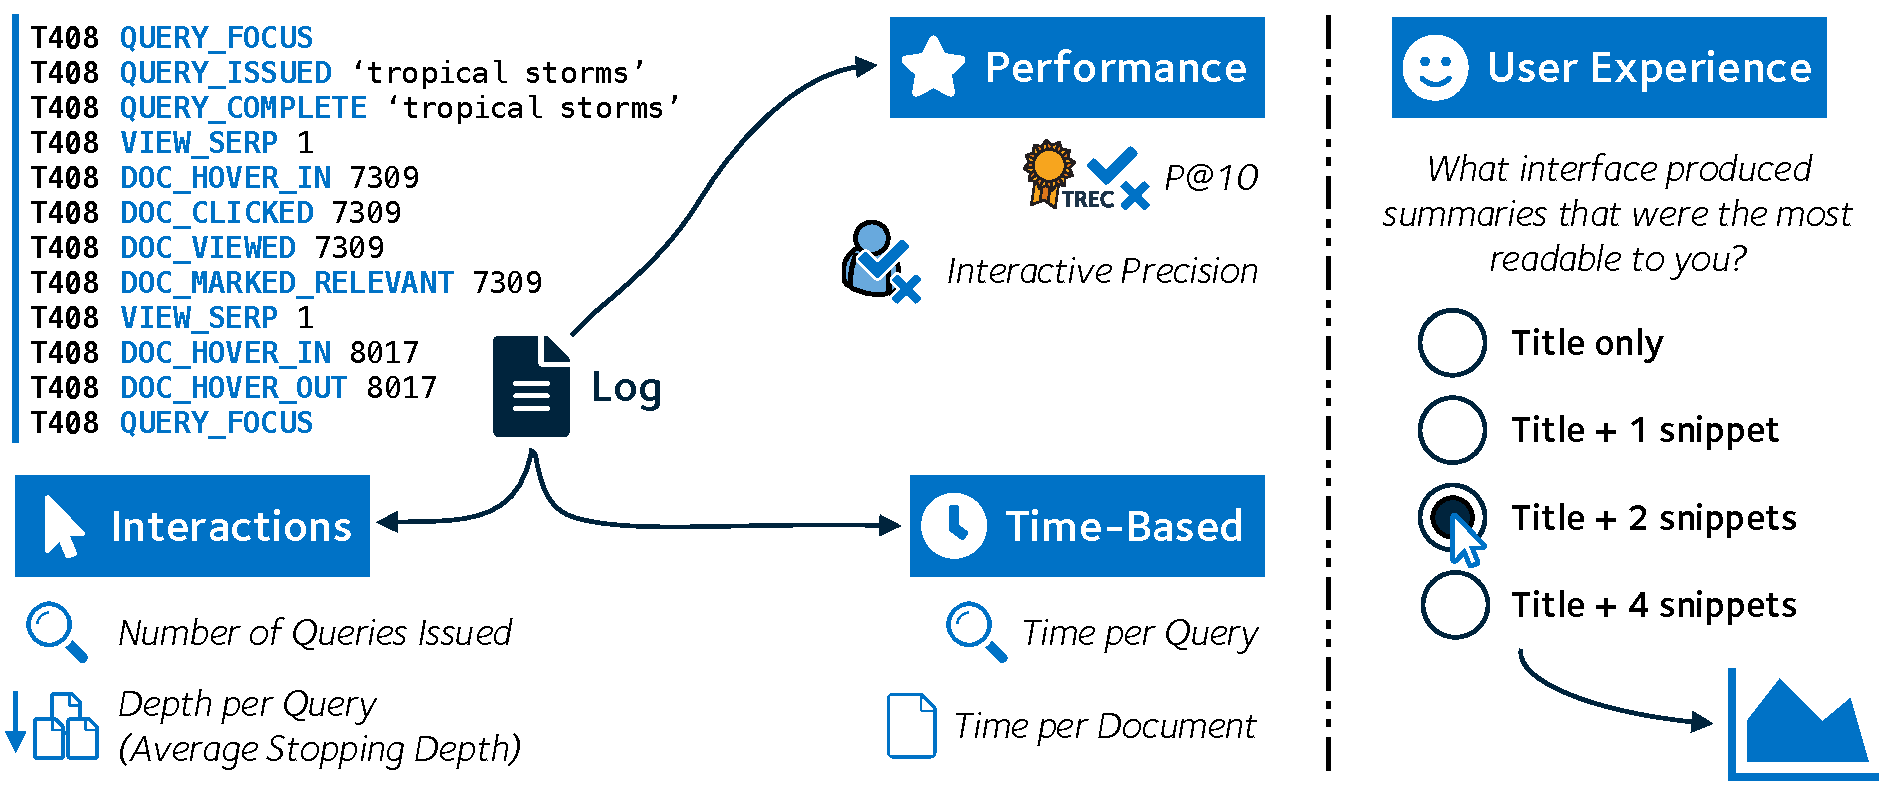
\includegraphics{figures/ch4-evaluation.pdf}}
    \caption[Examples of Evaluation Measures]{An illustration of the different types of measures that are captured, and from what sources. Interaction, time-based and performance measures are derived from the user study experiment log (with TREC QRELs used in conjunction with the interaction log to compute a subject's performance). User experience metrics are collated from a number of different surveys. Refer to Section~\ref{sec:csm:methodology:extracting} for more information.}
    \label{fig:evaluation_methodology}
\end{figure}

\subsubsection{Basic Interactions}
- recorded from log data.
- a number of different behavioural measures were recorded!

- clicks
- hovers
- and from that, the click depths. only click depths -- see time-based measures for an explanation as to why this is the case.
- number of queries
- number of documents marked

- list from the papers.

\subsubsection{Time-Based Measures}
- from the log data, as mentioned above, we also derived a number of time based measures.

- calculated from the point at which a searcher clicks or whatever, to the point they begin to do something else.

- query time -- from focus, to issuance.

- document time -- from clicking on a document, to returning to the~\gls{acr:serp}.

- per snippet time -- originally calculated from hover events. however, this in both studies proved to be unreliable.
- events triggered an AJAX callback...these came back to the server in a different order from which they were sent from the client, in a random order. as such, logging was inconsistent. and difficult to parse, unreliable.

- so made assumptions instead. we instead looked purely at the click depths for stopping -- and ignored hovers. use these for stopping depths.

\subsubsection{Performance Measures}
- as shown from figure~\ref{}, we were also able to extract a number of performance measures, too.
- using the raw data extracted from the interaction log file, we could, in conjunction with an additional evaluation tool (i.e. trec\_eval), use these two resources to calculate measures.

- measures that we considered across both studies included:

- P@10 -- query-based measures
- interactive precision and recall
- considering things too like number of documents marked, yet are not relevant.

- used in conjunction with behavioural measures, formed the basis of the seeded experiments.

\subsubsection{User Experience}
- not strictly necessary to forming a grounded simulation.
- but included to ascertain whether subjects perceived a difference between the interfaces and conditions trialled across the two experiments.

- split into five main parts:
    - demographics
    - pre-experiment
    - pre-task
    - post-task
    - post-experiment

- as previously mentioned, many of these components differed across the two studies that were undertaken. as such, we leave explanation of these surveys to each of the chapters.

\subsection{Simulating Searcher Behaviours}\label{chap:csm:method:simulation}
Simulation as defined earlier is a good means for experimentation.
Low cost, always use the same users, no issue of learning bias, etc.

EXPLORE how people's behaviours change

- set up the probabilities
- instantiate the components

- pick a topic set
- pick a corpus
- basic structure of the methodology from previous papers

\subsubsection{Instantiating the Simulations}

\subsubsection{Performance Runs}

\subsubsection{Comparison Runs}

\subsection{Evaluation of Simulations}\label{chap:csm:method:evaluation}
- how do we evaluate how good the system performs?
- how do we work out which one approximates best? on average.

\subsubsection{Determining Simulated User Performance}

\subsubsection{Comparing Simulated and Real-World Subjects}

\section{Chapter Summary}